\section{Reflection, endpoints, and the central value}\label{sec:endpoints}
\subsection{Limits on the full interior interval}\label{sec:interior-transport}
\Needspace{18\baselineskip}
\begin{lemma}[A specified reduction word and its scale factor]\label{lem:specified-reduction-word}
Let $m\in\Z_{\ge3}$. Let
\[
 \lambda_\pm=\frac{m\pm\sqrt{m^2-4}}2,\qquad
 I=(\lambda_-,\lambda_+),\qquad
 T(t)=\frac1{m-t},\qquad
 z(t)=\frac{t-\lambda_-}{\lambda_+-t}\quad(t\in I).
\]
Define the iterates by $T^0(t)=t$ and $T^{j+1}(t)=T(T^j(t))$ for $j\in\Z_{\ge0}$. Then, the following statements hold.

\begin{enumerate}
\item\label{c:reduction-cross-ratio} The maps $t\mapsto\frac1t$, $t\mapsto m-t$, and $T$ preserve $I$. The function $z$ is positive and strictly increasing on $I$. We have
\[
z(1)=\lambda_-,\qquad z(m-1)=\lambda_+,\qquad
z(T^j(t))=\lambda_+^{-2j}z(t)
\quad(t\in I,\ j\in\Z_{\ge0}).
\]
In particular,
\begin{equation}\label{eq:reduction-iterate}
T^j(t)=
\frac{\lambda_-+\lambda_+^{1-2j}z(t)}{1+\lambda_+^{-2j}z(t)}.
\end{equation}

\item\label{c:reduction-first-index} For $r\in I$, define
\[
\nu=\begin{cases}1,&r<1,\\0,&r\ge1,\end{cases}
\qquad
s=\begin{cases}\frac1r,&\nu=1,\\r,&\nu=0,\end{cases}
\]
\[
A=\frac{\log(\frac{z(s)}{\lambda_+})}{2\log\lambda_+},\qquad
N=\max\{0,\lceil A\rceil\},\qquad x=T^N(s),
\]
\[
\varepsilon=\begin{cases}1,&x>\frac m2,\\0,&x\le \frac m2,\end{cases}
\qquad
r_*=\begin{cases}m-x,&\varepsilon=1,\\x,&\varepsilon=0.\end{cases}
\]
Then, $N\in\Z_{\ge0}$, $1\le x\le m-1$, and $1\le r_*\le \frac m2$. Moreover,
\[
N=\min\{j\in\Z_{\ge0}:T^j(s)\le m-1\}.
\]

\item\label{c:reduction-word-scale} Use $\nu$, $N$, $\varepsilon$, and $r_*$ from Claim~\ref{c:reduction-first-index}. Define the integer matrices
\[
S=\begin{pmatrix}0&1\\1&0\end{pmatrix},\qquad
R=\begin{pmatrix}1&0\\m&-1\end{pmatrix},\qquad
G=R^\varepsilon(SR)^N S^\nu=(G_{ij})_{i,j\in[2]_{\Z}}.
\]
For $t\in I$, define
\begin{equation}\label{eq:reduction-scale-map}
c_G(t)=G_{11}+G_{12}t,\qquad
\rho_G(t)=\frac{G_{21}+G_{22}t}{G_{11}+G_{12}t}.
\end{equation}
We have $G_{11}+G_{12}t>0$, $\rho_G(t)\in I$, and $\rho_G(r)=r_*$. Both functions are continuous on $I$. If $(a,b)\in\cA_m$ and $t=\frac ba\in I$, define
\[
\binom{\widetilde a}{\widetilde b}=G\binom ab.
\]
Then,
\[
(\widetilde a,\widetilde b)\in\cA_m,\qquad
E_m(\widetilde a,\widetilde b)=E_m(a,b),\qquad
\frac{\widetilde a}{a}=c_G(t),\qquad
\frac{\widetilde b}{\widetilde a}=\rho_G(t).
\]
In particular, $c_m(r):=c_G(r)>0$ depends only on $m$ and $r$. If $r\in[1,\frac m2]$, then $G$ is the identity matrix, $c_m(r)=1$, and $r_*=r$.
\end{enumerate}
\end{lemma}
\begin{proof}
\prf{Claim~\ref{c:reduction-cross-ratio}} Let us use $\lambda_\pm=\frac{m\pm\sqrt{m^2-4}}2$. We have
\[
 \lambda_-+\lambda_+=m,\qquad \lambda_-\lambda_+=1,
 \qquad 0<\lambda_-<1<m-1<\lambda_+<m.
\]
For the strict inequality $m-1<\lambda_+$, evaluate the polynomial $t^2-mt+1$ at $m-1$: its value is $2-m<0$. Thus, $m-1$ lies between the two roots. The other inequalities follow from their positivity, product one, and sum $m>2$. Consequently, if $t\in I$, then
\[
 \lambda_-<\frac1t<\lambda_+,\qquad
 \lambda_-<m-t<\lambda_+.
\]
Their composition $T(t)=\frac1{m-t}$ also belongs to $I$. We have $m-t>0$.

Let us check that the change of variable is strictly increasing.
For $\lambda_-<u<v<\lambda_+$,
\[
 z(v)-z(u)=
 \frac{(\lambda_+-\lambda_-)(v-u)}{(\lambda_+-v)(\lambda_+-u)}>0.
\]
For $t\in I$, we have $t-\lambda_->0$ and $\lambda_+-t>0$. The identities $\lambda_-\lambda_+=1$ and $\lambda_-+\lambda_+=m$ give
\[
 z(1)=\frac{1-\lambda_-}{\lambda_+-1}=\lambda_-,\qquad
 z(m-1)=\frac{\lambda_+-1}{1-\lambda_-}=\lambda_+.
\]
They also give
\[
 \begin{aligned}
 z(T(t))
 &=\frac{1-(m-t)\lambda_-}{(m-t)\lambda_+-1}\\
 &=\frac{\lambda_-(t-\lambda_-)}{\lambda_+(\lambda_+-t)}
 =\lambda_+^{-2}z(t).
 \end{aligned}
\]
Induction on $j$ gives $z(T^j(t))=\lambda_+^{-2j}z(t)$. Solving $z(u)=\frac{u-\lambda_-}{\lambda_+-u}$ gives
\[
 u=\frac{\lambda_-+\lambda_+z(u)}{1+z(u)}.
\]
Substituting $u=T^j(t)$ and $z(T^j(t))=\lambda_+^{-2j}z(t)$ proves~\eqref{eq:reduction-iterate}.

\prf{Claim~\ref{c:reduction-first-index}} Let us verify the specified stopping index. Claim~\ref{c:reduction-cross-ratio} gives $s\in I$ and $s\ge1$. Since $z(s)>0$ and $\lambda_+>1$, the real number $A$ is defined. For every integer $j\ge0$, Claim~\ref{c:reduction-cross-ratio} and strict monotonicity of $z$ give
\[
 \begin{aligned}
 T^j(s)\le m-1
 &\Longleftrightarrow\lambda_+^{-2j}z(s)\le\lambda_+\\
 &\Longleftrightarrow j\ge A.
 \end{aligned}
\]
Therefore, $N=\max\{0,\lceil A\rceil\}$ is exactly the least nonnegative integer with $T^N(s)\le m-1$. If $N=0$, then $x=s\ge1$. If $N\ge1$, minimality gives $y:=T^{N-1}(s)>m-1$, while $y\in I$ gives $y<m$. Hence,
\[
 0<m-y<1,\qquad x=\frac1{m-y}>1.
\]
This proves $x\in[1,m-1]$. If $x\le \frac m2$, then $r_*=x\in[1,\frac m2]$. If $x>\frac m2$, then
\[
 1\le m-x<\frac m2,
\]
so $r_*=m-x\in[1,\frac m2]$.

\prf{Claim~\ref{c:reduction-word-scale}} Let us factor $G=R^\varepsilon(SR)^N S^\nu$. Put $d=\nu+2N+\varepsilon$. Define matrices $L_i$, $i\in[d]_{\Z}$, in application order by
\begin{equation}\label{eq:reduction-factor-indices}
 \begin{gathered}
 L_1=S\quad\text{if }\nu=1,\\
 L_{\nu+2j-1}=R,\quad L_{\nu+2j}=S\quad(j\in[N]_{\Z}),\\
 L_d=R\quad\text{if }\varepsilon=1.
 \end{gathered}
\end{equation}
The index ranges in~\eqref{eq:reduction-factor-indices} are disjoint and cover $[d]_{\Z}$. We have $G=L_d\cdots L_1$. For $d=0$, this product is the identity. For $t\in I$, put $t_0=t$ and, for $i\in[d]_{\Z}$, define
\[
 t_i=\begin{cases}\frac1{t_{i-1}},&L_i=S,\\m-t_{i-1},&L_i=R.\end{cases}
\]

Let us compute the first coordinate after applying $G$.
Claim~\ref{c:reduction-cross-ratio} gives $t_i\in I$ for $i\in[0,d]_{\Z}$.
For $i\in[d]_{\Z}$ and $a>0$, we have
\[
 S\binom{a}{at_{i-1}}=at_{i-1}\binom{1}{1/t_{i-1}},\qquad
 R\binom{a}{at_{i-1}}=a\binom{1}{m-t_{i-1}}.
\]
Both first coordinates are positive since $t_{i-1}\in I\subset(0,m)$.
Starting with $(1,t)^{\mathsf T}$ and applying $L_1,\ldots,L_d$ gives
\[
 c_G(t)=\prod_{\substack{i\in[d]_{\Z}\\L_i=S}}t_{i-1}>0,
 \qquad \rho_G(t)=t_d\in I.
\]
The empty product equals one.
The construction in Claim~\ref{c:reduction-first-index} gives $t_d=r_*$ when $t=r$.

Let us prove continuity of $c_G$ and $\rho_G$ at an arbitrary $t\in I$.
For any sequence $(t_n)_{n\ge1}$ in $I$ satisfying $\lim_{n\to\infty}t_n=t$, we have
\[
 \lim_{n\to\infty}(G_{11}+G_{12}t_n)=G_{11}+G_{12}t=c_G(t)>0.
\]
Equation~\eqref{eq:reduction-scale-map} and the quotient limit give
\[
 \lim_{n\to\infty}c_G(t_n)=c_G(t),\qquad
 \lim_{n\to\infty}\rho_G(t_n)
 =\frac{G_{21}+G_{22}t}{G_{11}+G_{12}t}=\rho_G(t).
\]

Let us identify the corresponding transformations of dimension pairs.
On integer dimension pairs the two factors act by
\[
 S\binom ab=\binom ba,\qquad
 R\binom ab=\binom a{ma-b}.
\]
Each intermediate pair is positive because its slope belongs to $I$. Claims~\ref{c:moduli-symmetries-identities}, \ref{c:moduli-coprimality}, and~\ref{c:moduli-quadratic} of Lemma~\ref{lem:moduli-symmetries} and~\eqref{eq:nonempty-domain} preserve membership in $\cA_m$ and the Euler characteristic at each step. More explicitly,
\[
 \gcd(b,a)=\gcd(a,b),\qquad \gcd(a,ma-b)=\gcd(a,b),
\]
\[
 m ba-b^2-a^2=mab-a^2-b^2,
\]
\[
 ma(ma-b)-a^2-(ma-b)^2=mab-a^2-b^2.
\]
The Euler identities are those of Claim~\ref{c:moduli-symmetries-identities} of Lemma~\ref{lem:moduli-symmetries}. Multiplication by $G$ gives
\[
 \frac{\widetilde a}{a}=G_{11}+G_{12}t=c_G(t),\qquad
 \frac{\widetilde b}{\widetilde a}
 =\frac{G_{21}+G_{22}t}{G_{11}+G_{12}t}=\rho_G(t).
\] If $1\le r\le \frac m2$, then $\nu=0$, $r\le m-1$, $N=0$, and $\varepsilon=0$. Thus, $G=\left(\begin{smallmatrix}1&0\\0&1\end{smallmatrix}\right)$, $c_m(r)=1$, and $r_*=r$.
\end{proof}

\begin{lemma}[Endpoint folding]\label{lem:reduction-endpoint-fold}
Let $m\in\Z_{\ge3}$, put $I=(\lambda_-,\lambda_+)$, and let $\rho\in[1,\frac m2]$. Define
\[
 \delta_\rho=
 \begin{cases}
 \frac12\min\{\rho-1,\frac m2-\rho\},&1<\rho<\frac m2,\\
 \frac{m-2}{2m},&\rho=1,\\
 \frac{m-2}{4},&\rho=\frac m2.
 \end{cases}
\]
The cases are disjoint because $m>2$. We have $\delta_\rho>0$. For $(a,b)\in\cA_m$, $t=\frac ba\in I$, and $|t-\rho|<\delta_\rho$, define
\[
 \operatorname{Fold}_\rho(a,b)=(a',b')=
 \begin{cases}
 (a,b),&1<\rho<\frac m2,\\
 (\min(a,b),\max(a,b)),&\rho=1,\\
 (a,\min(b,ma-b)),&\rho=\frac m2.
 \end{cases}
\]
Then,
\[
 (a',b')\in\cA_m,\qquad E_m(a',b')=E_m(a,b),\qquad
 1\le \frac{b'}{a'}\le \frac m2.
\]
Moreover, the ratios are exactly
\[
 \left(\frac{a'}a,\frac{b'}{a'}\right)=
 \begin{cases}
 (1,t),&1<\rho<\frac m2,\\
 (\min(1,t),\max(t,\frac1t)),&\rho=1,\\
 (1,\min(t,m-t)),&\rho=\frac m2.
 \end{cases}
\]
Consequently, let $((a_n,b_n))_{n\ge1}$ be a sequence in $\cA_m$ satisfying
\[
 \lim_{n\to\infty}\frac{b_n}{a_n}=\rho.
\]
Then, there is $N\in\Z_{>0}$ such that $\operatorname{Fold}_\rho(a_n,b_n)=(a'_n,b'_n)$ is defined for every $n\ge N$ and satisfies
\[
 (a'_n,b'_n)\in\cA_m,\qquad E_m(a'_n,b'_n)=E_m(a_n,b_n),\qquad 1\le\frac{b'_n}{a'_n}\le\frac m2.
\]
We have
\[
 \lim_{n\to\infty}\frac{a'_n}{a_n}=1,\qquad
 \lim_{n\to\infty}\frac{b'_n}{a'_n}=\rho.
\]
\end{lemma}
\begin{proof}
First, suppose $1<\rho<\frac m2$. Then,
\[
 1<\rho-\delta_\rho<t<\rho+\delta_\rho<\frac m2.
\]
The pair is unchanged. Thus, all conclusions follow.

Second, suppose $\rho=1$. The chosen radius satisfies
\[
 1-\delta_1=\frac{m+2}{2m}>\frac2m,
 \qquad
 1+\delta_1=\frac{3m-2}{2m}<\frac m2,
\]
where $\frac{3m-2}{2m}<\frac m2$ follows from $(m-1)(m-2)>0$. Therefore,
\[
 \frac2m<t<\frac m2,
 \qquad 1\le\max(t,\frac1t)<\frac m2.
\]
If $t\ge1$, then $\operatorname{Fold}_1(a,b)=(a,b)$. If $t<1$, then $\operatorname{Fold}_1(a,b)=(b,a)$. These two cases give
\[
 \frac{a'}a=\min(1,t),\qquad \frac{b'}{a'}=\max(t,\frac1t).
\]
Vertex exchange preserves membership in $\cA_m$ and the Euler characteristic by Claims~\ref{c:moduli-symmetries-identities}, \ref{c:moduli-coprimality}, and~\ref{c:moduli-quadratic} of Lemma~\ref{lem:moduli-symmetries} and~\eqref{eq:nonempty-domain}.

Third, suppose $\rho=\frac m2$. In this case
\[
 1<\frac{m+2}{4}=\rho-\delta_\rho<t
 <\rho+\delta_\rho=\frac{3m-2}{4}<m-1.
\]
Therefore,
\[
 1<\min(t,m-t)\le \frac m2.
\]
For $t\le \frac m2$, the pair $\operatorname{Fold}_{\frac m2}(a,b)$ equals $(a,b)$.
For $t>\frac m2$, it equals $(a,ma-b)$.
Thus, $\frac{a'}a=1$ and $\frac{b'}{a'}=\min(t,m-t)$.
Claims~\ref{c:moduli-symmetries-identities}, \ref{c:moduli-coprimality}, and~\ref{c:moduli-quadratic} of Lemma~\ref{lem:moduli-symmetries} and~\eqref{eq:nonempty-domain} give $(a',b')\in\cA_m$ and $E_m(a',b')=E_m(a,b)$.

Let us pass to the limit in each case. We have $[1,\frac m2]\subset I$. Convergence to $\rho$ puts $t_n=\frac{b_n}{a_n}$ in $I\cap(\rho-\delta_\rho,\rho+\delta_\rho)$ for all sufficiently large $n$. The limits $\frac{a'_n}{a_n}\to1$ and $\frac{b'_n}{a'_n}\to\rho$ follow from continuity of $\min$, $\max$, and inversion at a positive number. At $\rho=1$, these limits are $\min(1,1)=1$ and $\max(1,1)=1$. At $\rho=\frac m2$, the slope limit is $\min(\frac m2,m-\frac m2)=\frac m2$.
\end{proof}

\begin{lemma}[Reduction of sequences of dimension pairs]\label{lem:approaching-dimension-reduction}
Let $m\in\Z_{\ge3}$ and $r\in(\lambda_-,\lambda_+)$.
Then, there are numbers $r_*\in[1,\frac m2]$ and $c_m(r)>0$ depending only on $m$ and $r$ with the following property.
For each sequence $((a_n,b_n))_{n\ge1}$ in $\cA_m$ such that
\begin{equation}\label{eq:approaching-reduction-input}
 \lim_{n\to\infty}a_n=\infty,\qquad
 \lim_{n\to\infty}\frac{b_n}{a_n}=r,
\end{equation}
there are an integer $N\ge1$ and pairs $(a'_n,b'_n)\in\cA_m$ for $n\ge N$ such that
\begin{equation}\label{eq:approaching-reduction-pairs}
 1\le\frac{b'_n}{a'_n}\le\frac m2,\qquad
 E_m(a'_n,b'_n)=E_m(a_n,b_n)\qquad(n\ge N),\qquad\text{and}
\end{equation}
\begin{equation}\label{eq:approaching-reduction-limits}
 \frac{a'_n}{a_n}\longrightarrow c_m(r),\qquad
 \frac{b'_n}{a'_n}\longrightarrow r_*\qquad(n\longrightarrow\infty).
\end{equation}
\end{lemma}
\begin{proof}
Let us apply one fixed reduction word to the sequence.
Put $I=(\lambda_-,\lambda_+)$. Let $G$, $r_*$, and $c_m(r)=G_{11}+G_{12}r>0$ be the objects specified in Lemma~\ref{lem:specified-reduction-word}. By~\eqref{eq:approaching-reduction-input}, the slopes $\frac{b_n}{a_n}$ belong to $I$ for all sufficiently large $n$. For these indices, define
\[
 \binom{\widetilde a_n}{\widetilde b_n}=G\binom{a_n}{b_n}.
\]
Claim~\ref{c:reduction-word-scale} of Lemma~\ref{lem:specified-reduction-word} gives
\[
 \begin{gathered}
 (\widetilde a_n,\widetilde b_n)\in\cA_m,
 \qquad E_m(\widetilde a_n,\widetilde b_n)=E_m(a_n,b_n),\\
 \frac{\widetilde a_n}{a_n}
 =G_{11}+G_{12}\frac{b_n}{a_n}\longrightarrow c_m(r),\\
 \frac{\widetilde b_n}{\widetilde a_n}
 =\frac{G_{21}+G_{22}(\frac{b_n}{a_n})}{G_{11}+G_{12}(\frac{b_n}{a_n})}
 \longrightarrow r_*.
 \end{gathered}
\]
Apply Lemma~\ref{lem:reduction-endpoint-fold} with $\rho=r_*$. Define
\[
 (a'_n,b'_n)=\operatorname{Fold}_{r_*}(\widetilde a_n,\widetilde b_n)
\]
for $n\ge N$, where $N\ge1$ is large enough for Lemma~\ref{lem:reduction-endpoint-fold} to apply. That lemma gives $(a'_n,b'_n)\in\cA_m$, $E_m(a'_n,b'_n)=E_m(\widetilde a_n,\widetilde b_n)$, and $1\le\frac{b'_n}{a'_n}\le\frac m2$. Thus~\eqref{eq:approaching-reduction-pairs} holds. Lemma~\ref{lem:reduction-endpoint-fold} gives
\[
 \frac{a'_n}{a_n}
 =\frac{a'_n}{\widetilde a_n}\frac{\widetilde a_n}{a_n}
 \longrightarrow1\cdot c_m(r)=c_m(r),
 \qquad \frac{b'_n}{a'_n}\longrightarrow r_*.
\]
This proves~\eqref{eq:approaching-reduction-limits}. The definitions of $G$, $r_*$, and $c_m(r)$ use only $m$ and $r$.
\end{proof}

\begin{proposition}\label{prop:interior-limit}
For every integer $m\ge3$, there is a function
$F_m:(\lambda_-,\lambda_+)\to(0,\infty)$ such that the following hold.
\begin{enumerate}
\item\label{c:interior-limit} We have
\[
 \lim_{\substack{a\to\infty,\ (a,b)\in\cA_m\\\frac{b}{a}\to r}}
 \frac{\log E_m(a,b)}a=F_m(r)
 \qquad\bigl(r\in(\lambda_-,\lambda_+)\bigr).
\]
\item\label{c:interior-continuity} The function $F_m$ is continuous.
\end{enumerate}
\end{proposition}
\begin{proof}
\prf{Claim~\ref{c:interior-limit}} Let us first obtain the limit for $r\in[1,\frac m2]$.
Fix such an $r$ and consider $(a,b)\in\cA_m$ such that
\[
 a\longrightarrow\infty,\qquad \frac ba\longrightarrow r,\qquad
 1\le\frac ba\le\frac m2.
\]

First, let us obtain the limit when $m\ge4$.
Define $\Upsilon_m(1)=\ell(R_1)$ and $\Upsilon_m(m-2)=\ell(R_{m-2})$.
For all sufficiently large $a$, we have $b>a\ge2$ and
$1<\Gamma(a,b)<\frac ba\le \frac{m}{2}\le m-2$ by~\eqref{eq:ambient}.
The floor differences in~\eqref{eq:frame-word} and the appended simple run have vertical lengths in $[m-2]_{\Z}$.
Claims~\ref{c:integer-limit} and~\ref{c:integer-endpoints} of Proposition~\ref{prop:integer},
Theorem~\ref{thm:rational}, and Theorem~\ref{thm:irrational-large-m} give the limits on $[1,\frac{m}{2}]$.
Lemma~\ref{lem:word-bounds} and~\eqref{eq:dictionary} give positivity.

Second, let us obtain the limit when $m=3$.
Theorem~\ref{thm:rational}, Claim~\ref{c:three-irrational-limit} of
Proposition~\ref{prop:three-irrational}, and Corollary~\ref{cor:central} give the limits on $[1,\frac32]$.
Claim~\ref{c:three-irrational-continuity} of Proposition~\ref{prop:three-irrational} gives positivity.
Thus, the positive limits on $[1,\frac m2]$ equal $\Upsilon_m(r)$.

Let us obtain the limit at each $r\in(\lambda_-,\lambda_+)$.
Let $((a_n,b_n))_{n\ge1}$ be any sequence in $\cA_m$ satisfying
\[
 \lim_{n\to\infty}a_n=\infty,\qquad
 \lim_{n\to\infty}\frac{b_n}{a_n}=r.
\]
Apply Lemma~\ref{lem:approaching-dimension-reduction} to this sequence.
Since $\frac{a'_n}{a_n}\to c_m(r)>0$, we have $a'_n\to\infty$.
Hence,
\[
 \frac{\log E_m(a_n,b_n)}{a_n}
 =\frac{a'_n}{a_n}\frac{\log E_m(a'_n,b'_n)}{a'_n}
 \longrightarrow c_m(r)\Upsilon_m(r_*)>0.
\]

Let us define $F_m$ on $(\lambda_-,\lambda_+)$.
The numbers $r_*$ and $c_m(r)$ depend only on $m$ and $r$.
Lemma~\ref{lem:approaching-sequence} supplies at least one sequence approaching $r$.
Define $F_m(r)$ to be the common limit of $\frac1{a_n}\log E_m(a_n,b_n)$ along all such sequences.
Then,
\[
 F_m(r)=c_m(r)\Upsilon_m(r_*)
 \qquad\bigl(r\in(\lambda_-,\lambda_+)\bigr).
\]
For $r\in[1,\frac{m}{2}]$, Claim~\ref{c:reduction-word-scale} of Lemma~\ref{lem:specified-reduction-word}
gives $r_*=r$ and $c_m(r)=1$.
Thus, Claim~\ref{c:interior-limit} holds at every interior slope.

Let us identify $F_m(r)$ with $\Upsilon_m(r)$ on the entire interval $(1,M_{\mathrm{run}}(m))$.
Fix $r$ in this interval and choose a sequence $((a_n,b_n))_{n\ge1}$ as in~\eqref{eq:approaching-sequence}.

If $m\ge4$ and $r$ is an integer, equations~\eqref{eq:ambient} and~\eqref{eq:frame-word} give $(a_n,b_n)\in\mathcal S_m$ for all sufficiently large $n$.
Claim~\ref{c:integer-limit} of Proposition~\ref{prop:integer} and~\eqref{eq:rational-period} then give the limit $\Upsilon_m(r)=\ell(R_r)$.

For noninteger rational $r$, Theorem~\ref{thm:rational} and~\eqref{eq:rational-period} give the limit $\Upsilon_m(r)$.
For irrational $r$, Theorem~\ref{thm:irrational-large-m} applies when $m\ge4$, and Claim~\ref{c:three-irrational-limit} of Proposition~\ref{prop:three-irrational} applies when $m=3$.

Comparing each limit with Claim~\ref{c:interior-limit} gives
\[
 F_m(r)=\Upsilon_m(r)\qquad\bigl(1<r<M_{\mathrm{run}}(m)\bigr).
\]

Let $r\in(\lambda_-,\lambda_+)$.
First, let us prove $F_m(r)=rF_m(1/r)$.
By Lemma~\ref{lem:approaching-sequence}, choose a sequence $((a_n,b_n))_{n\ge1}$ in $\cA_m$ satisfying
\[
 \lim_{n\to\infty}a_n=\infty,\qquad
 \lim_{n\to\infty}\frac{b_n}{a_n}=r.
\]
Since $r>0$, we have $b_n\to\infty$ and $\frac{a_n}{b_n}\to\frac1r$.
Claim~\ref{c:moduli-symmetries-identities} of Lemma~\ref{lem:moduli-symmetries} gives
\[
 \frac{\log E_m(a_n,b_n)}{a_n}
 =\frac{b_n}{a_n}\frac{\log E_m(b_n,a_n)}{b_n}
 \longrightarrow rF_m\left(\frac1r\right).
\]

Second, let us prove $F_m(r)=F_m(m-r)$.
Since $m-r>0$, choose $n_0\in\Z_{>0}$ such that
\[
 m-\frac{b_n}{a_n}>\frac{m-r}{2}>0\qquad(n\ge n_0).
\]
Thus, $ma_n-b_n>0$ for $n\ge n_0$, and
\[
 \frac{ma_n-b_n}{a_n}\longrightarrow m-r,\qquad
 \frac{\log E_m(a_n,b_n)}{a_n}
 =\frac{\log E_m(a_n,ma_n-b_n)}{a_n}
 \longrightarrow F_m(m-r).
\]
Both transformed sequences belong to $\cA_m$ by Lemma~\ref{lem:moduli-symmetries}
and~\eqref{eq:nonempty-domain}. Comparing these limits with Claim~\ref{c:interior-limit} gives
\begin{equation}\label{eq:entropy-symmetries}
 F_m(r)=rF_m\left(\frac1r\right),\qquad F_m(r)=F_m(m-r).
\end{equation}

\prf{Claim~\ref{c:interior-continuity}} Let us prove continuity at each interior slope.
Let $r\in(\lambda_-,\lambda_+)$ and choose
$\lambda_-<h_1<r<h_2<\lambda_+$.
Claim~\ref{c:interior-limit} and Lemma~\ref{lem:approaching-sequence} verify the hypotheses of
Lemma~\ref{lem:continuity} for $F_m|_{[h_1,h_2]}$.
Claim~\ref{c:continuity-function} of Lemma~\ref{lem:continuity} gives continuity at $r$.
\end{proof}

\subsection{\texorpdfstring{Proof of Theorem~\ref{thm:main} and upper bound}{Proof of Theorem 1.1 and upper bound}}
\begin{proof}[Proof of Theorem~\ref{thm:main}]
Let us prove the limit of $\frac1a\log E_m(a,b)$ at both endpoints.
Claim~\ref{c:interior-limit} of Proposition~\ref{prop:interior-limit} gives positivity and~\eqref{eq:main-limit}
on $(\lambda_-,\lambda_+)$. Let $F_m(\lambda_\pm)=0$.
Fix $r\in\{\lambda_-,\lambda_+\}$ and any sequence $((a_n,b_n))_{n\ge1}$ in $\cA_m$ such that
$a_n\to\infty$ and $r_n=\frac{b_n}{a_n}\to r$.
Since $mr-1-r^2=0$, we have
\[
 \max(mr_n-1-r_n^2,0)\longrightarrow0,
 \qquad
 \frac{\log(\frac{2^m}{m})}{a_n}\longrightarrow0
 \qquad(n\to\infty).
\]
The bound~\eqref{eq:finite-endpoint} gives
\[
 0\le\frac{\log E_m(a_n,b_n)}{a_n}
 \le m\log2\sqrt{\frac{m+2}{m-2}}\sqrt{\max(mr_n-1-r_n^2,0)}
   +\frac{\log(\frac{2^m}{m})}{a_n}\longrightarrow0.
\]
Thus, we obtain
\eqref{eq:main-limit} for $r=\lambda_-$ and $r=\lambda_+$.

Let us prove continuity on the closed interval $I_m$.
For every $r\in I_m$, Lemma~\ref{lem:approaching-sequence} supplies a sequence satisfying~\eqref{eq:approaching-sequence}.
Apply Claim~\ref{c:continuity-function} of Lemma~\ref{lem:continuity} with $J=I_m=[\lambda_-,\lambda_+]$.
\end{proof}

\begin{corollary}[Quantitative upper bound]\label{cor:upper-bound}
For each integer $m\ge3$, the function $F_m$ in
Theorem~\ref{thm:main} satisfies
\begin{equation}\label{eq:main-bound}
 F_m(r)\le m\log2\sqrt{\frac{m+2}{m-2}}
       \sqrt{(\lambda_+-r)(r-\lambda_-)}
       \qquad(r\in I_m).
\end{equation}
\end{corollary}
\begin{proof}
Let us obtain~\eqref{eq:main-bound} from~\eqref{eq:finite-endpoint}.
For $r\in(\lambda_-,\lambda_+)$, choose a sequence $((a_\nu,b_\nu))_{\nu\ge1}$ in $\cA_m$ satisfying~\eqref{eq:approaching-sequence}.
Put $r_\nu=\frac{b_\nu}{a_\nu}$. Equations~\eqref{eq:main-limit} and~\eqref{eq:finite-endpoint} give
\[
 \begin{aligned}
 F_m(r)
 &=\lim_{\nu\to\infty}\frac{\log E_m(a_\nu,b_\nu)}{a_\nu}\\
 &\le\lim_{\nu\to\infty}\left(
 m\log2\sqrt{\frac{m+2}{m-2}}\sqrt{\max(mr_\nu-1-r_\nu^2,0)}
 +\frac{\log(\frac{2^m}{m})}{a_\nu}\right)\\
 &=m\log2\sqrt{\frac{m+2}{m-2}}\sqrt{mr-1-r^2}.
 \end{aligned}
\]
The identity $mr-1-r^2=(\lambda_+-r)(r-\lambda_-)$ proves~\eqref{eq:main-bound}.
For $r=\lambda_\pm$, both sides are zero.
\end{proof}

\subsection{The value at slope one and some figures for \texorpdfstring{$F_m$}{Fm}}
\begin{corollary}\label{cor:central-value}
For every $m\ge3$,
\begin{equation}\label{eq:central-value}
 \begin{aligned}
 \lim_{\substack{a\to\infty,\ (a,b)\in\cA_m\\\frac{b}{a}\to1}}
 \frac{\log E_m(a,b)}a
 &=F_m(1)\\
 &=(m-1)^2\log((m-1)^2)-m(m-2)\log(m(m-2)).
 \end{aligned}
\end{equation}
\end{corollary}
\begin{proof}
Let us obtain the limit along dimensions $(a,a+1)$.
The adjacent-dimension formula of~\cite[Theorem 6.6]{Weist} is
\[
 E_m(a,a+1)=\frac{m}{(a+1)((m-1)a+m)}
          \binom{(m-1)^2a+(m-1)m}{a}.
\]
Fix $m$ and let $c=(m-1)^2$ and $d=m(m-1)$.
Stirling's formula $\log(n!)=n\log n-n+O(\log n)$ gives, as $a\to\infty$ through positive integers,
\[
 \begin{aligned}
 \log\binom{ca+d}{a}
 &=(ca+d)\log(ca+d)-a\log a\\
 &\quad-((c-1)a+d)\log((c-1)a+d)+O(\log a)\\
 &=a\bigl(c\log c-(c-1)\log(c-1)\bigr)+O(\log a).
 \end{aligned}
\]
The constants in the error terms depend only on $m$.
For the prefactor, we have
\[
 \log\frac{m}{(a+1)((m-1)a+m)}=-2\log a+O(1).
\]
Dividing by $a$ gives
\[
 \begin{aligned}
 \frac1a\log\binom{ca+(m-1)m}{a}
 &\longrightarrow c\log c-(c-1)\log(c-1),\\
 \frac1a\log\frac{m}{(a+1)((m-1)a+m)}&\longrightarrow0.
 \end{aligned}
\]
Since $c-1=m(m-2)$, equation~\eqref{eq:main-limit} gives~\eqref{eq:central-value}.
\end{proof}




\begin{figure}[H]
\centering
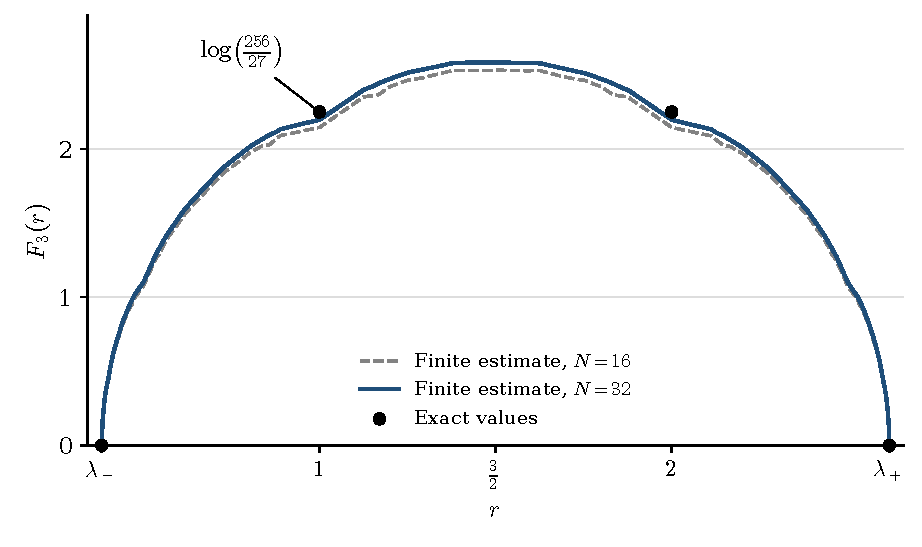
\includegraphics[width=\textwidth]{figures/f3-figure.pdf}
\caption[Numerical illustration of $F_3$]{Numerical illustration of $F_3$ on $I_3$.
Here $\lambda_\pm=\frac{3\pm\sqrt5}{2}$.
For each reduced $\alpha=\frac pq\in[1,\frac32]$ with $q\le8$,
let $N\in\{16,32\}$ and $j=\floor{\frac Nq}$. We use
$\widehat F_N(\alpha)=
\frac{\log C_0(W_{p,q}^{2j})-\log C_0(W_{p,q}^j)}{jq}$.
We interpolate these values linearly and extend them by
\eqref{eq:entropy-symmetries}. The dots mark the exact values
$F_3(\lambda_\pm)=0$ and
$F_3(1)=F_3(2)=\log\left(\frac{256}{27}\right)$.
The curves are finite approximations; we do not assert an error bound.}
\label{fig:f3}
\end{figure}


\begin{figure}[H]
\centering
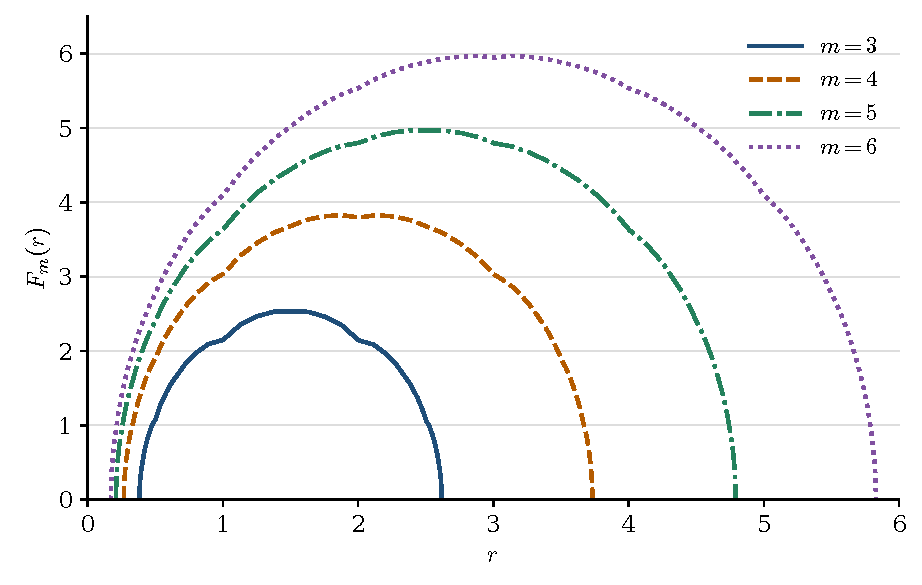
\includegraphics[width=\textwidth]{figures/fm-figure.pdf}
\caption[Finite approximations for $m=3$, $4$, $5$, and $6$]{Finite approximations to
$F_m(r)$ for $m=3$, $4$, $5$, and $6$, each on its interval $I_m$.
For $\alpha=1+\frac{k}{8}$ with $k\in[0,4(m-2)]_{\Z}$, let
$\alpha=\frac pq$ in lowest terms and let $j=\frac{16}{q}$.
We evaluate $C_0$ for the indicated $m$ and use
$\widehat F_m(\alpha)=
\frac{\log C_0(W_{p,q}^{2j})-\log C_0(W_{p,q}^j)}{jq}$.
We interpolate these values linearly on $[1,\frac m2]$ and extend them by
\eqref{eq:entropy-symmetries}. We use the exact value zero at both endpoints.
The curves are finite approximations; we do not assert an error bound.}
\label{fig:fm-comparison}
\end{figure}

